\documentclass[twoside, letterpaper, 12pt]{report}
\usepackage{orthodoxservicebook}

\title{The Sunday Reader's Service of the \\ \textsc{Typica} \\ 2020 April 26}
\titlepic{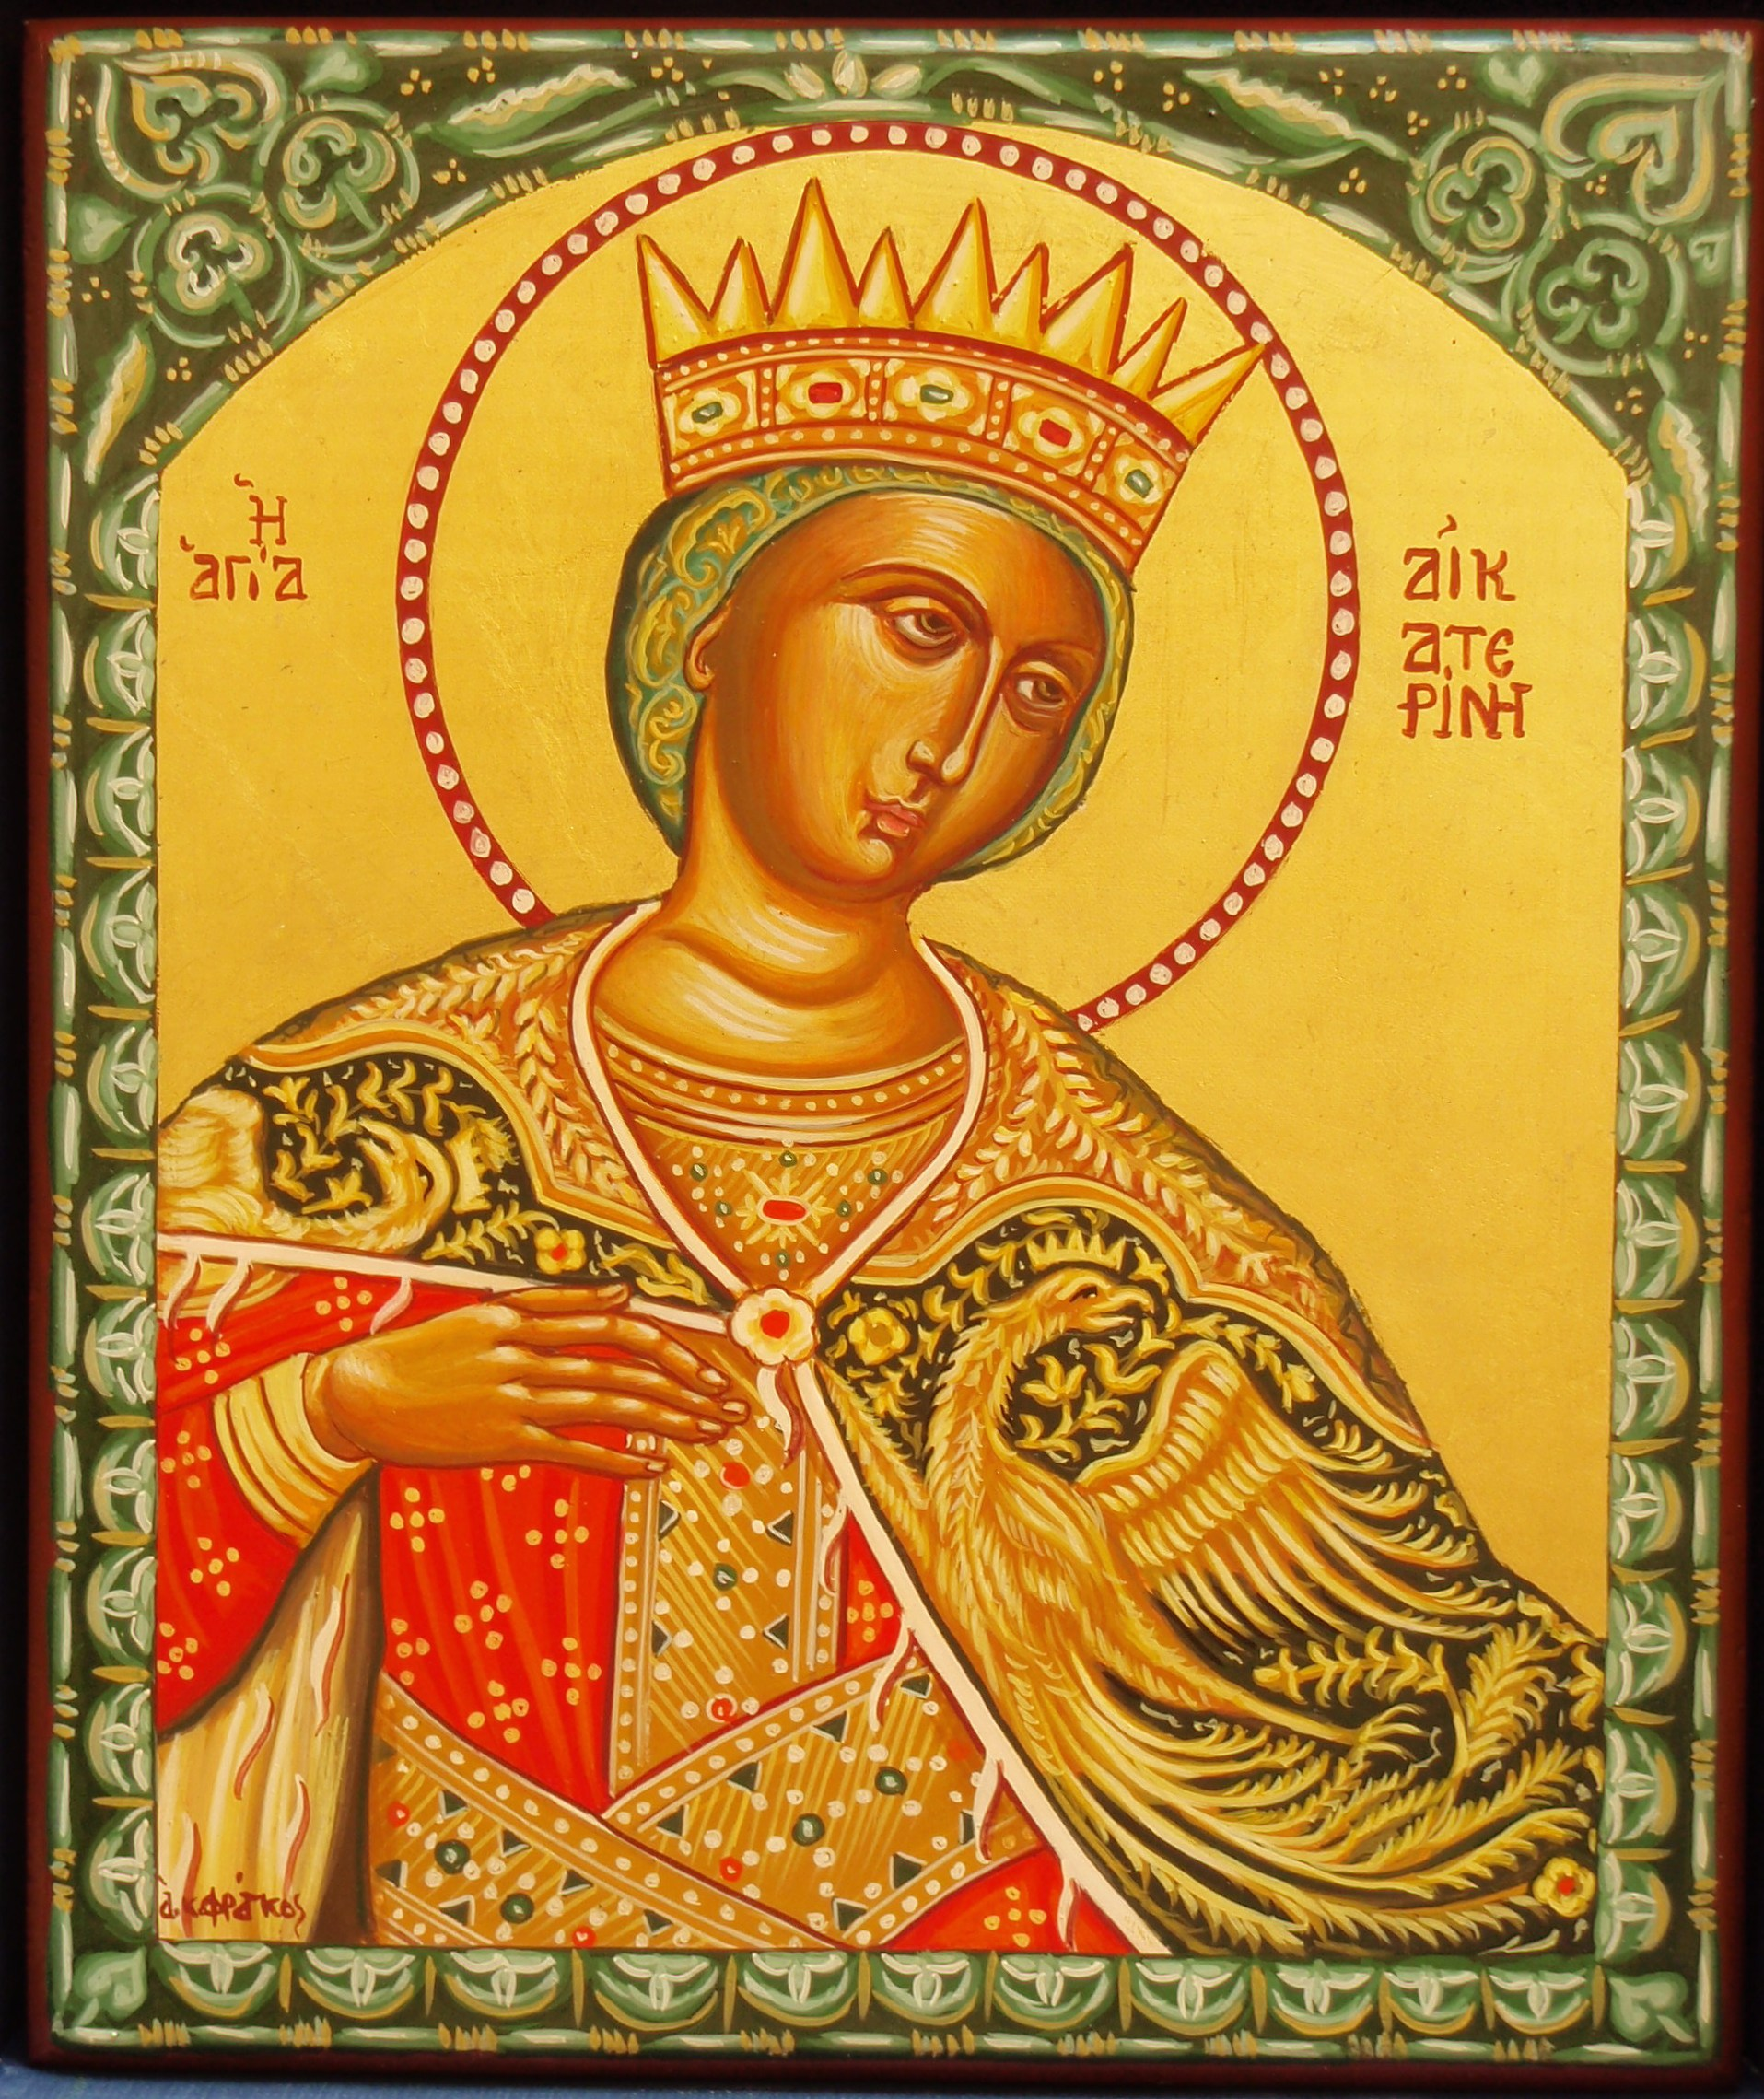
\includegraphics[width=0.5\textwidth]{Katherine1.jpg}}
\date{}
\author{}

\begin{document}
\maketitle
\pagestyle{empty} % Don't show page numbers
\instruction{This page intentionally left blank}
\cleardoublepage
\pagestyle{plain}
\setcounter{page}{1} % Set the page counter to 1 on the first real page
\chapter*{Service of Typica on Sunday, April 26 \\
          New Sunday or Anti-Pascha\\
          Sunday of Thomas the Apostle, called "The Twin"}

\readerline{\throughtheprayers{}}
\lilypondfile{./Z-Responses/Obikhod/Amen.ly}

\trisagionNeedsAmen[reader][prepentecost]

\lilypondfile{./Z-Responses/Obikhod/Amen.ly}


\centeredsection{The First Antiphon}
\lilypondfile{./Liturgy/B-FirstAntiphon/BlessTheLord_Greek-Music.ly}

\centeredsection{The Second Antiphon}
\lilypondfile{./Liturgy/C-SecondAntiphon/PraiseTheLord_Greek-Music.ly}

\centeredsection{The Third Antiphon}
\lilypondfile{./Liturgy/D-ThirdAntiphon/Beatitudes_Moscow-Music.ly}

\centeredsection{The Epistle}

\instruction{Both of the New Testament lessons are read
without liturgical introduction or conclusion.
The readers start with “The Reading from…” and proceeds}

\paragraph{The Reading from the Acts of the Saintly and Pure Apostles. (5:12-20)}\mbox{}\\

\begin{maybetwocolumns}
In those days, many signs and wonders were done among the people by the hands of the
Apostles. And they were all together in Solomon’s Portico. None of the rest dared join them, but
the people held them in high honor. And more than ever believers were added to the Lord,
multitudes both of men and women, so that they even carried out the sick into the streets, and laid
them on beds and pallets, that as Peter came by at least his shadow might fall on some of them.
The people also gathered from the towns around Jerusalem, bringing the sick and those afflicted
with unclean spirits, and they were all healed. But the high priest rose up and all who were with
him, that is, the party of the Sadducees, and filled with jealousy they arrested the Apostles and put
them in the common prison. But at night an angel of the Lord opened the prison doors and brought
them out and said, “Go and stand in the temple and speak to the people all the words of this Life.”
\end{maybetwocolumns}

\centeredsection{The Gospel}

\instruction{Both of the New Testament lessons are read
without liturgical introduction or conclusion.
The readers start with “The Reading from…” and proceeds}

\paragraph{The Reading from the Holy Gospel according to St. John. (20:19-31)}\mbox{}\\

\begin{maybetwocolumns}
On the evening of that day, the first day of the week, the doors being shut where the
Disciples were, for fear of the Jews, Jesus came and stood among them and said to them, “Peace
be with you.” When He had said this, He showed them His hands and His side. Then the Disciples
were glad when they saw the Lord. Jesus said to them again, “Peace be with you. As the Father
has sent me, even so I send you.” And when He had said this, He breathed on them, and said to
them, “Receive the Holy Spirit. If you forgive the sins of any, they are forgiven; if you retain the
sins of any, they are retained.” Now Thomas, one of the Twelve, called the Twin, was not with
them when Jesus came. So the other Disciples told him, “We have seen the Lord.” But he said to
them, “Unless I see in His hands the print of the nails, and place my finger in the mark of the nails,
and place my hand in His side, I will not believe.” Eight days later, His Disciples were again in
the house, and Thomas was with them. The doors were shut, but Jesus came and stood among
them, and said, “Peace be with you.” Then He said to Thomas, “Put your finger here, and see My
hands; and put out your hand, and place it in my side; do not be faithless, but believing.” Thomas
answered Him, “My Lord and my God!” Jesus said to him, “Have you believed because you have
seen Me? Blessed are those who have not seen and yet believe.” Now Jesus did many other signs
in the presence of the Disciples, which are not written in this book; but these are written that you
may believe that Jesus is the Christ, the Son of God, and that believing you may have life in His
Name.
\end{maybetwocolumns}

\centeredsection{Troparia Before the Creed}
\instruction{Plain reading}
\begin{reader}
\item[Reader 1:] The heavenly choir singeth thy praises, saying:
  Holy, holy, holy, Lord of Sabaoth; heaven and earth are full of Thy glory.

\item[Reader 2:] \emph{Come unto him, and be enlightened,
               and your faces shall not be ashamed.}
  The heavenly choir singeth thy praises, saying:
  Holy, holy, holy, Lord of Sabaoth; heaven and earth are full of Thy glory.

\item[Reader 1:] \emph{\glory}
  The choir of the holy angels and archangels,
  with all the powers of heaven, singeth thy praises, saying:
  Holy, holy, holy, Lord of Sabaoth; heaven and earth are full of Thy glory.

\item[Reader 2:]\emph{\nowandever}
\end{reader}

\centeredsection{The Creed}
\input{Common/TheCreed.txt}


\centeredsection{Prayer of Forgiveness}
\readerline{Forgive, remit, pardon, O God, our sins,
  both voluntary and involuntary, in deed and in word, in knowledge or in ignorance,
  committed by night or by day, in mind and in thought.
  Forgive us them all, for thou art good and lovest mankind.
}


\centeredsection{The Lord’s Prayer}
\input{Common/LordsPrayer.txt}

\readerline{Through the prayers of our holy fathers, Lord Jesus Christ our God, have mercy on us.}
\lilypondfile{./Z-Responses/Obikhod/Amen.ly}


\centeredsection{Kontakia for Pascha in Tone 8}

Though Thou didst descend into the grave, O Immortal One, yet didst Thou destroy the power of
Hades, and didst arise as victor, O Christ God, calling to the myrrh-bearing women, Rejoice, and
giving peace unto Thine Apostles, O Thou Who dost grant resurrection to the fallen.


\readerline{\lhmForty}

\readerline{
  O Christ our God, Who art worshipped and glorified at all times at every hour both in
  heaven and on earth; Who art long-suffering and plenteous in mercy and compassion; Who lovest
  the just man and showest mercy upon the sinner; and Who callest all men to repentance through 
  the promise of blessings to come; receive, O Lord, at this very hour our supplications, and direct
  our lives in the way of Thy commandments: sanctify our souls, purify our bodies, set our minds
  aright, cleanse our thoughts; deliver us from all affliction, trouble, and distress; compass us about
  with Thy holy angels, that, guided and guarded by them, we may attain unto the unity of the Faith,
  and to the knowledge of Thine unapproachable glory; for Thou art blessed unto ages of ages. Amen.
}

\begin{reader}
  \item \lhmThree{}\\\emph{\gne{}}
  \item \morehonorablethanthetherubim{}
  \item \throughtheprayers{}
\end{reader}

\begin{maybetwocolumns}
\lilypondfile{./Z-Responses/Obikhod/Amen.ly}

\readerline{\blessedbethename{}\thrice{}}

\centeredsection{Psalm 33}
\input{./Psalms/Psalm033-unknowntrans.txt}

\centeredsection{Psalm 144}
\input{./Psalms/Psalm144-unknowntrans.txt}
\end{maybetwocolumns}

\peopleline{\gne}


\centeredsection{A Homily}
\begin{maybetwocolumns}
\instruction{Sunday after Pascha, 6th Sunday of Quarantine\\
His Bodily Wounds and Ours: Homily for Thomas Sunday in the Orthodox Church
Fr. Philip LeMasters, pastor, St. Luke Antiochian Orthodox Church of Abilene, Texas}

I was surprised a few years ago in one of my college classes when even the best students
were surprised to learn that Christian hope for eternal life includes the resurrection of the body.
They were comfortable thinking of human souls experiencing eternal life, but doubted that our
actual physical bodies would have any part in the Kingdom of Heaven. Especially on this Sunday
of St. Thomas, we celebrate how Christ’s bodily resurrection is the basis of hope for our own.
Today we proclaim that our Savior brings healing and transformation to whole, embodied persons,
for that is how He conquered death on the third day.

As we continue to celebrate the glorious good news of this season of Pascha, we recall how Christ
called doubting Thomas to faith in His great victory. “He said to Thomas, ‘Put your finger here,
and see My hands; and put out your hand, and place it in my side; do not be faithless, but believing.’
Thomas answered Him, ‘My Lord and my God!’” Still bearing His wounds even in His glorified
body as the God-Man, the Risen Christ brought Thomas to faith through the witness of His own
deified flesh.

We have probably heard the story so many times that we have become deaf to its importance.
Nonetheless, it remains the case that the Savior’s resurrection is not an escape from the body or
the physical world, but instead their healing and sanctification. Likewise, St. John referred in his
epistle to that “which we have seen with our own eyes, which we have looked upon and touched
with our hands, concerning the word of life—the life was made manifest, and we saw it…” The
Apostles saw the Lord after His resurrection with their eyes, touched Him with their hands, heard
His voice with their ears, felt His breath on their skin, and even saw Him eat food. (Luke 24: 36-
43) The good news that “God is light and in Him is no darkness at all” comes from a resurrection
in glory of a complete Person with a human body marked by the wounds of torture and crucifixion.
His resurrection is not an escape from the body, but its fulfillment. The Eternal Word Who created
us by breathing into the dust of the earth now breathes physically on His Disciples as He empowers
them to carry out His ministry of bringing salvation to the world, even to the point of forgiving
sins in His name. Here are powerful signs of what it means for human beings to be in the likeness
of God and partakers of the divine nature by grace.

These are not merely details of ancient history, but reminders that we participate in Christ’s
Passover from death to life by how we live as whole, embodied persons. We were baptized
physically with water into Christ’s death in order to put Him on like a garment, in order to rise
with Him into a new life of holiness. To be blunt, the Christian life is not simply about our
emotions, ideas, or opinions; it is not reduced to what we say we believe. For those who are truly
in Christ will live in ways that manifest the brilliant life of the resurrection, that radiate the holy
light of the Savior’s great victory over sin and death. As St. John put it, “If we say we have
fellowship with Him while we walk in darkness, we lie and do not live according to the truth; but
if we walk in the light, as He is in the light, we have fellowship with one another, and the blood of
Jesus His Son cleanses us from all sin.”

We participate in the new life of our Risen Lord by walking into His light, by embracing as fully
as we can the blessed healing of the human being that He has brought to the world. Christ’s
Passion was not a matter simply of His feelings, words, or ideas, but of His complete Self-offering
through crucifixion, burial, descent to Hades, and resurrection from the dead. He rises in glory
with His wounds, and we cannot begin to make sense of His salvation without speaking of the
most bodily of realities, such as torture, execution, death, and burial in a tomb that was later found
to be empty.

We are probably all tempted at times to think how much easier it would be to serve God if we did
not have our particular set of bodily limitations and problems. Some are challenged by physical
or mental illness, while others wrestle with passions for the pleasures of food, sex, alcohol, or other
substances. Eating disorders and unrealistic expectations of what their bodies should look like
ruin the health and well-being of some, while others struggle to accept that their male or female
bodies are signs of who they are in God’s image and likeness. Many today ignore the sacredness
of the intimate bodily union of man and woman, which makes two into one flesh. The epidemic
of pornography in our culture reflects a repudiation of the sacredness of the flesh and blood through
which we encounter the living icons of Christ. Some refuse to honor the bodies of their neighbors
by becoming blind to the humanity of children in the womb, of people with skin of a different
color, or of terminally ill patients in chronic pain. And whether it is greed, sloth, anger, or refusal
to help the needy with our time, attention, and resources, there is no sin that does not show itself
physically in some way in the lives of those who struggle with it.

No matter what someone’s particular struggles, weaknesses, or failings are, we must respond with
compassion, for we too are among the sick who need the Physician. Nonetheless, no physical
condition can ever make us sin or do evil. The problem is not that we have bodies, but that we
choose to remain in the tomb, that we would rather walk in the darkness than in the light. For it is
no sin to be ill or to be tempted in any way. The Lord Himself suffered terribly on the cross and
was tempted. It is a sin, however, to let any of our wounds become excuses for not walking in the
light as best we can. It is a sin to let anything fill our lives with such darkness that we refuse to
open our eyes—and our lives—to the good news of the resurrection. It is a sin when we think that
God must remove this or that problem in order to earn our faithfulness, in order to be worthy of
our devotion. As we celebrate Christ’s great victory over sin and death, we must not be afraid to
expose our wounded selves to Him with humility as we say with St. Thomas “’My Lord and my
God!’”

Remember that the Savior has taken upon Himself even the worst bodily wounds. It is through
them that He has brought life out of death and brilliant light out of the darkest tomb. He has
conquered even death itself. Do you see what that means? Even our darkest inclinations ultimately
do not stand a chance against His glory, if we will only expose them to Him, if we will only offer
them to Him for healing. And though it probably will not happen instantaneously, our wounds
will find healing as we move step by step further into His light. Darkness is simply the absence
of light and it disappears when it is illumined. The same Lord Who conquered Hades and the tomb
for our salvation, and Who invited Thomas to touch His wounds, will bring us as whole, embodied
persons into the new day of His Kingdom if we will only keep turning as best we can from the
darkness as we struggle to live faithfully each day in the midst of the problems, pains, and
weaknesses that beset us. We must all take that journey one day at a time.

The good news is that Christ does not ask us to conquer sin and death by our own power, for He
has already done that. But He does ask us truly to have faith, which requires a faithful life, even
as we constantly ask for His mercy and strength to participate as fully as possible in the joy of His
resurrection. We will not do that with a fake spirituality that relies purely on emotions or ideas,
but as whole persons of flesh and blood enlivened by the One Who made us in His image and
likeness and even died and rose again for our salvation. So let us celebrate Pascha by walking in
the light as best we can with all our wounds, for that is how we will open ourselves to the light
that has made even the tomb radiant with the divine glory. If He can do that to a grave, just imagine
what He can do with us.
\end{maybetwocolumns}

\centeredsection{Apolytikion for Thomas Sunday in Tone 7}
While the tomb was sealed, Thou didst shine forth from it, O Life. While the doors were closed,
Thou didst come in to Thy Disciples, O Christ God, Resurrection of all, renewing in us through
them an upright spirit, according to the greatness of Thy mercy.

\centeredsection{Megalynarion for Thomas Sunday in Tone 1}
O most radiant lamp, the Theotokos, the immeasurable honor, which is more exalted than all
creatures, with praises do we magnify thee.

\vspace{1cm}
\instruction{If your family chooses to process around the exterior of your house,
you can sing the Apolytikia of Lazarus Saturday and Palm Sunday,
“Rejoice, O Bethany” and the Trisagion Hymn}

\readerline{\throughtheprayers}

\lilypondfile{./Z-Responses/Obikhod/Amen.ly}

\end{document}

